\documentclass[8pt, a4paper, oneside, twocolumn]{extarticle}
\usepackage{graphicx}
\usepackage[export]{adjustbox}
\usepackage[compact]{titlesec}  % documentation: http://mirror.iopb.res.in/tex-archive/macros/latex/contrib/titlesec/titlesec.pdf  
\usepackage{kotex}
\usepackage[left=0.8cm, right=0.8cm, top=2cm, bottom=0.3cm, a4paper]{geometry}
\usepackage{amsmath}
\usepackage{ulem}
\usepackage{amssymb}
\usepackage{minted}  % syntax highlighting
\usepackage{enumitem}
\setlist{nolistsep}
\usepackage{fancyhdr} % documentation: http://ctan.math.utah.edu/ctan/tex-archive/macros/latex/contrib/fancyhdr/fancyhdr.pdf
\usepackage{lastpage}  % just so that we can use \pageref {LastPage}
\usepackage{color, hyperref}
% The lines in the table of contents become links to the corresponding pages in the document by simply adding in the preamble of the document the line
\usepackage{tikz}
\usetikzlibrary{positioning,chains,fit,shapes,calc}
\newcommand{\swastik}[1]{%
    \begin{tikzpicture}[#1]
        \draw (-1,1)  -- (-1,0) -- (1,0) -- (1,-1);
        \draw (-1,-1) -- (0,-1) -- (0,1) -- (1,1);
    \end{tikzpicture}%
}
\newcommand{\revised}{To be \textcolor{red}{\textbf{revised}}.}
\titlespacing*{\section}
{0pt}{0px plus 1px minus 0px}{-2px plus 0px minus 0px}
\titlespacing*{\subsection}
{0pt}{0px plus 1px minus 0px}{0px plus 3px minus 3px}
\titlespacing*{\subsubsection}
{0pt}{0px plus 1px minus 0px}{0px plus 3px minus 3px}
\setlength{\columnseprule}{0.4pt}
\DeclareRobustCommand{\stirling}{\genfrac\{\}{0pt}{}}
\setlength{\parindent}{0pt}  % so that there is no indent of paras.
\begin{document}
\title{\swastik {scale = 0.2} {}Compiler Short Revision Notes{} \swastik {scale = 0.2}}
\author{Sourabh Aggarwal}
\date{Compiled on \today}
\maketitle
\pagenumbering{roman}
\tableofcontents
\newpage
\thispagestyle{fancy}  % else it was not giving fancy header to the first page
\pagenumbering{arabic}
\section{Intro}
Lexical means relating to the words or vocabulary of a language.

Most useful abstraction are context free grammer for parsing and regular expressions for lexical analysis. Yacc which converts a grammer into a parsing program, Lex which converts a declarative specification into lexical analysis program. 

Useful resource: \href{https://www.cs.princeton.edu/~appel/modern/ml/}{Click}

Language of straight line programs:

The informal semantics of the language is as follows. Each $Stm$ is a 
statement, each $Exp$ is an expression. $s_1;s_2$ executes statement $s_1$, then statement
$s_2$. i:=e evaluates the expression e, then "stores" the result in variable i.

print ($e_1, e_2, \dots, e_n$) displays the values of all the expressions, evaluated
left to right, separated by spaces, terminated by a newline.
An identifier expression, such as i, yields the current contents of the 
variable i. A number evaluates to the named integer. An operator expression
$e_1 \text{ op } e_2$ evaluates e1, then e2, then applies the given binary operator. And
an expression sequence (s, e) behaves like the C-language "comma" 
operator, evaluating the statement s for side effects before evaluating (and returning
the result of) the expression e.
For example, executing this program
a := 5+3; b := (print(a, a-1), 10*a); print(b)
prints

8 7

80

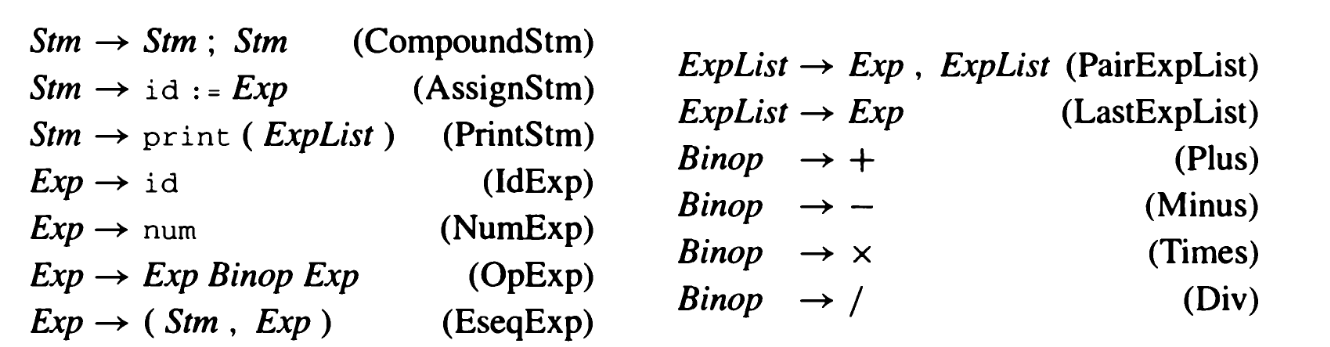
\includegraphics[width=0.5\textwidth,height=0.5\textheight,keepaspectratio]{slpg}

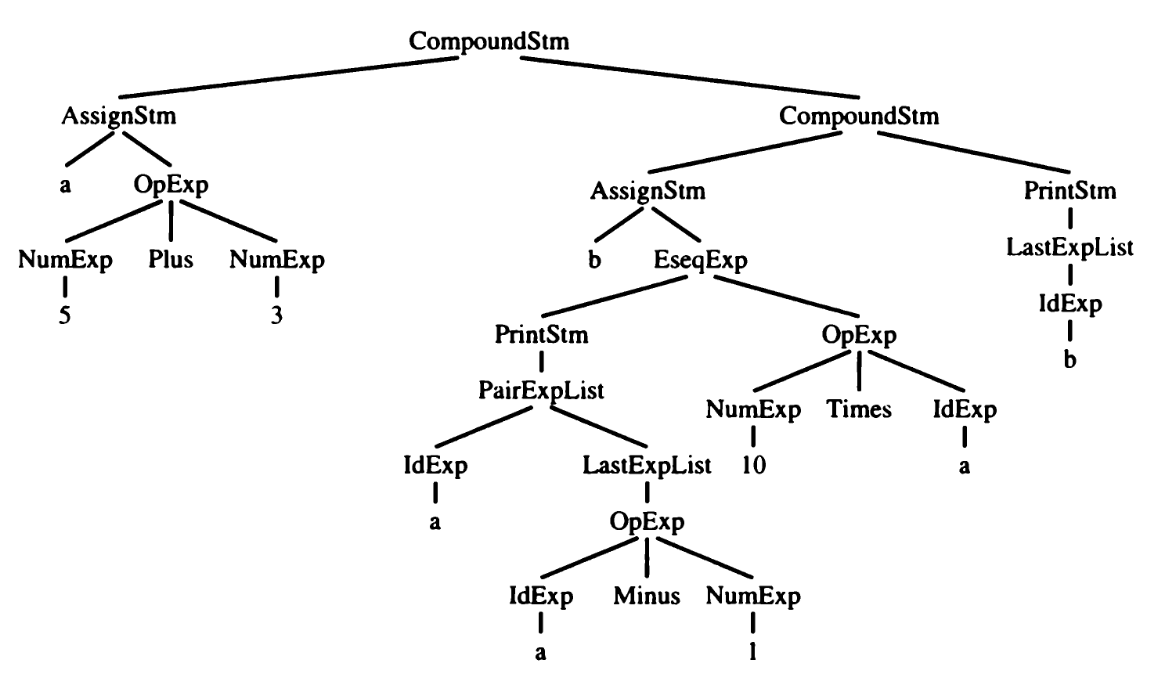
\includegraphics[width=0.5\textwidth,height=0.5\textheight,keepaspectratio]{slpt}

\begin{minted}{SML}
type id = string
datatype binop = Plus | Minus | Times | Div
datatype stm = CompoundStm of stm * stm
             | AssignStm of id * exp
             | PrintStm of exp list
     and exp = IdExp of id
             | NumExp of int
             | OpExp of exp * binop * exp
             | EseqExp of stm * exp
\end{minted}
To translate a program from one language into another, a compiler must first 
pull it apart and understand its structure and meaning, then put it together in a 
different way. The front end of the compiler performs analysis; the back end 
does synthesis. 
The analysis is usually broken up into 
Lexical analysis: breaking the input into individual words or "tokens";The lexical analyzer takes a stream of characters and produces a stream of 
names, keywords, and punctuation marks;  it discards white space and comments between the tokens. 

Syntax analysis: parsing the phrase structure of the program; and 

Semantic analysis: calculating the program's meaning. 

we will specify lexical tokens using the formal language of regular 
expressions, implement lexers using deterministic finite automata, and use 
mathematics to connect the two. This will lead to simpler and more readable 
lexical analyzers. 
$(a \odot b) \vert \epsilon$ represents the language \{""," ab"\}. 
In writing regular expressions, we will sometimes omit the concatenation 
symbol or the epsilon, and we will assume that Kleene closure "binds tighter" 
than concatenation, and concatenation binds tighter than alternation; so that 
$ab \vert c$ means $(a \odot b) \vert c$, and $(a \vert)$ means $(a \vert \epsilon)$. 
Let us introduce some more abbreviations: [abed] means 
$(a \vert b \vert c \vert 
d)$, [b-g] means [bedefg], [b-gM-Qkr] means [bcdefgMNOPQkr], M? 
means ($M \vert \epsilon$), and $M^+$ means ($M \odot M^*$). 

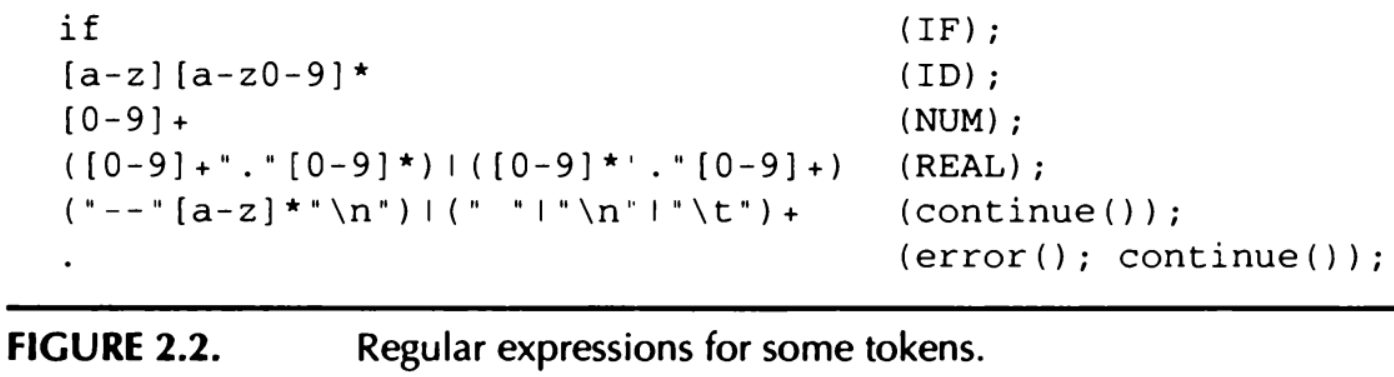
\includegraphics[width=0.5\textwidth,height=0.5\textheight,keepaspectratio]{reg}

Longest match: The longest initial substring of the input that can match any 
regular expression is taken as the next token. 

Rule priority: For a particular longest initial substring, the first regular  
expression that can match determines its token type. This means that the order of 
writing down the regular-expression rules has significance. 

So according to the rules, if8 match as a single 
identifier and not as the two tokens if and 8. And "if 89" begin with a 
reserved word and not by an identifier by rule priority rule. 

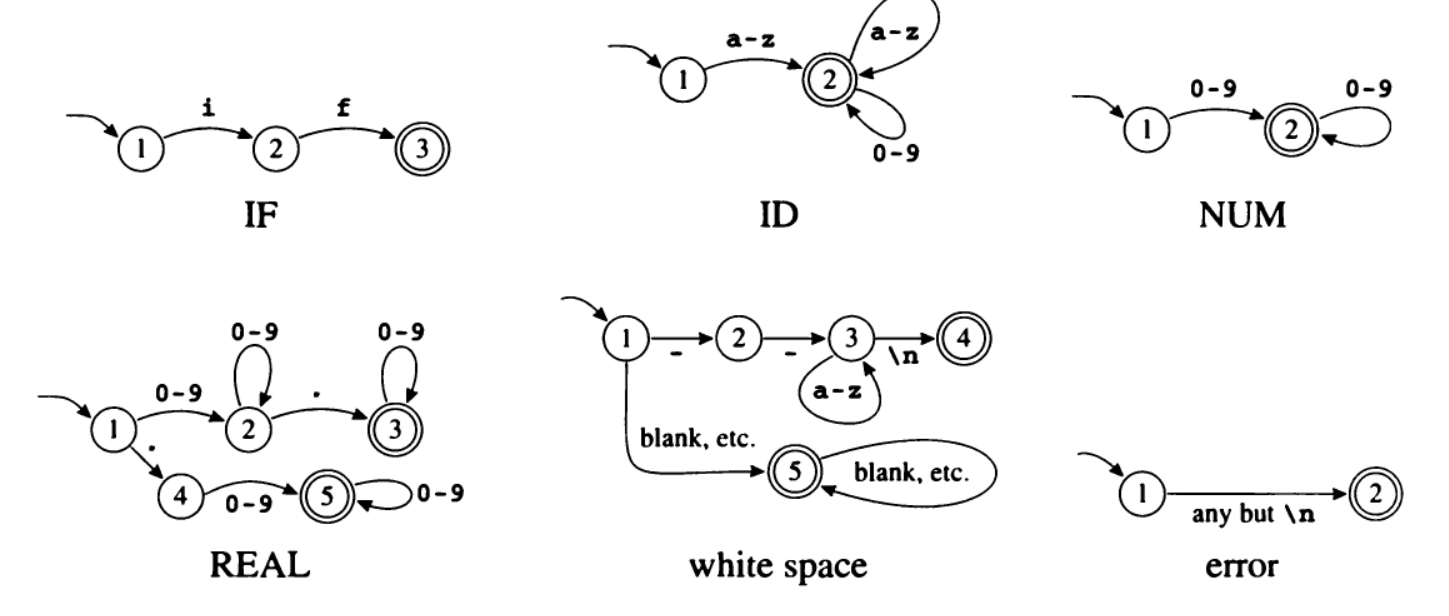
\includegraphics[width=0.5\textwidth,height=0.5\textheight,keepaspectratio]{aut}

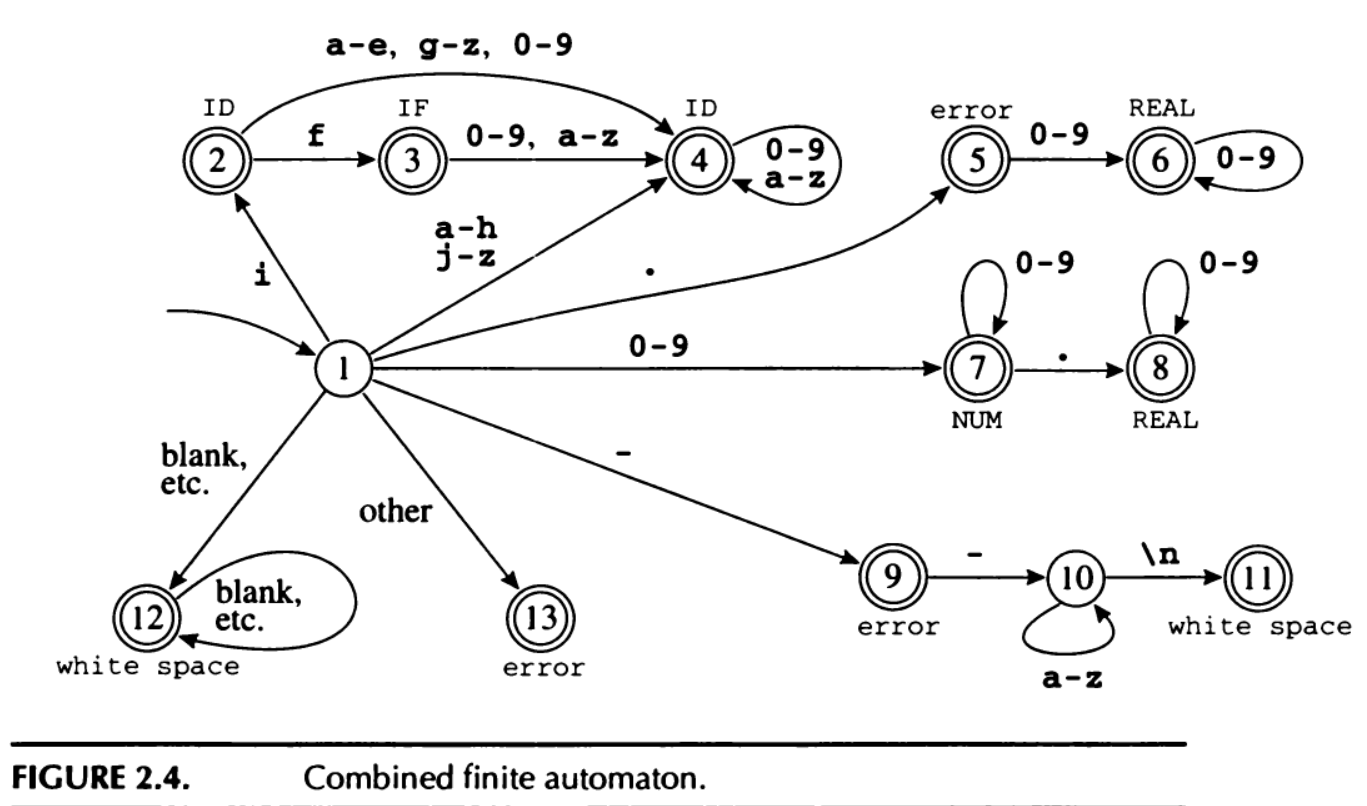
\includegraphics[width=0.5\textwidth,height=0.5\textheight,keepaspectratio]{cfa}

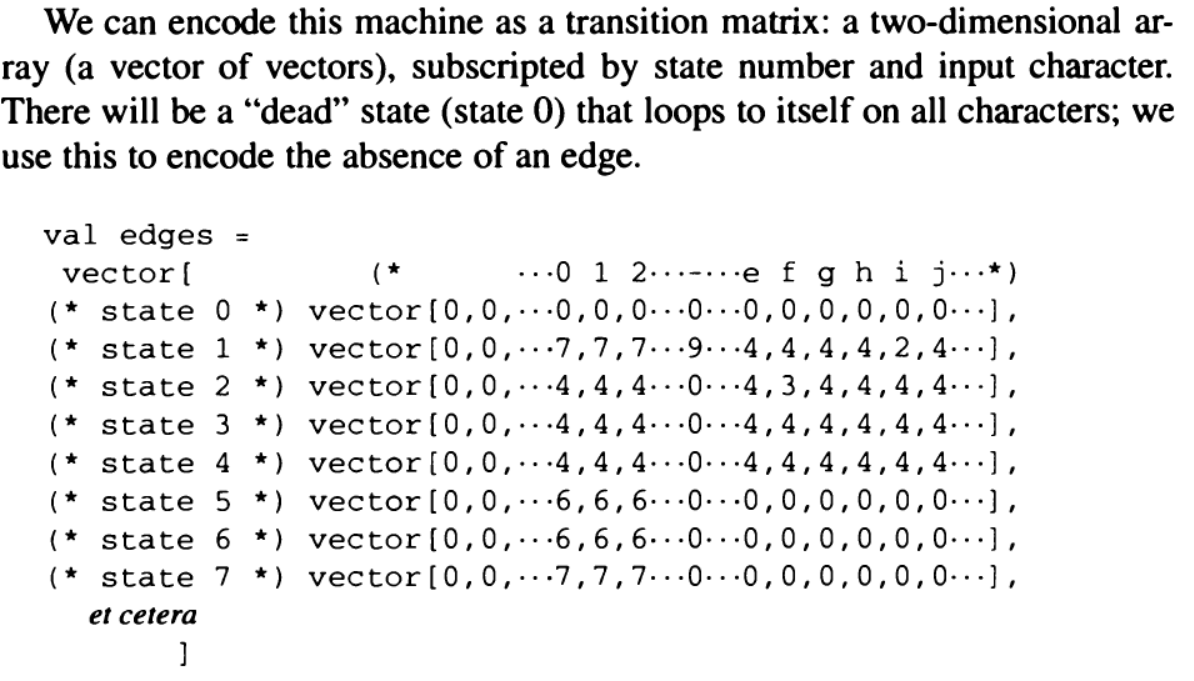
\includegraphics[width=0.5\textwidth,height=0.5\textheight,keepaspectratio]{mat}

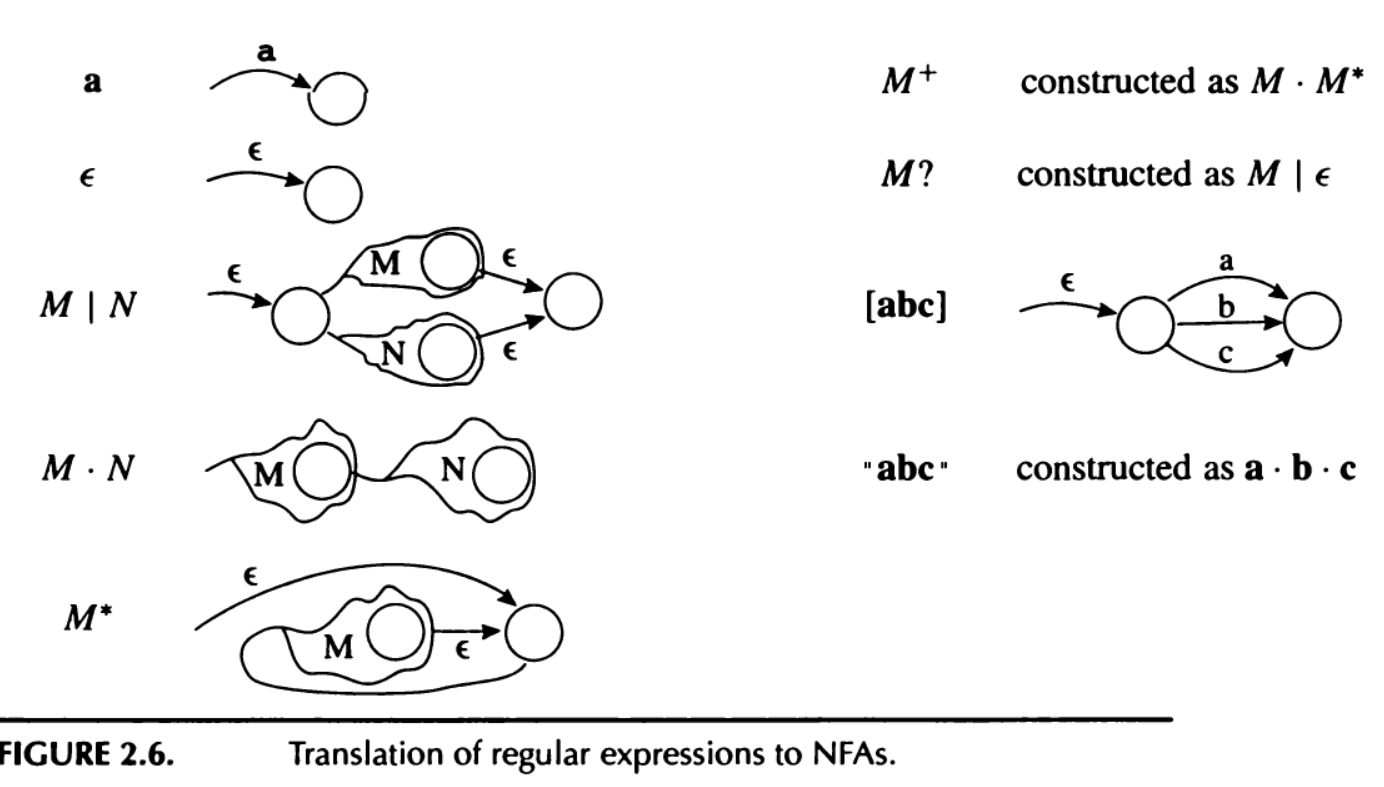
\includegraphics[width=0.5\textwidth,height=0.5\textheight,keepaspectratio]{rtnfa}

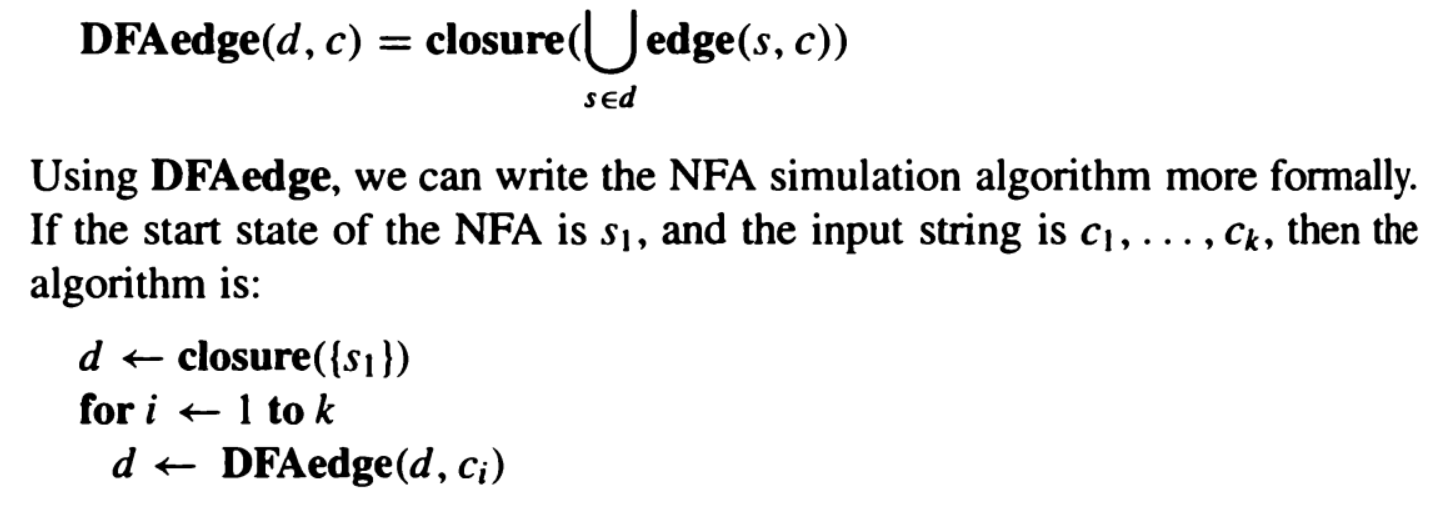
\includegraphics[width=0.5\textwidth,height=0.5\textheight,keepaspectratio]{nfa1}

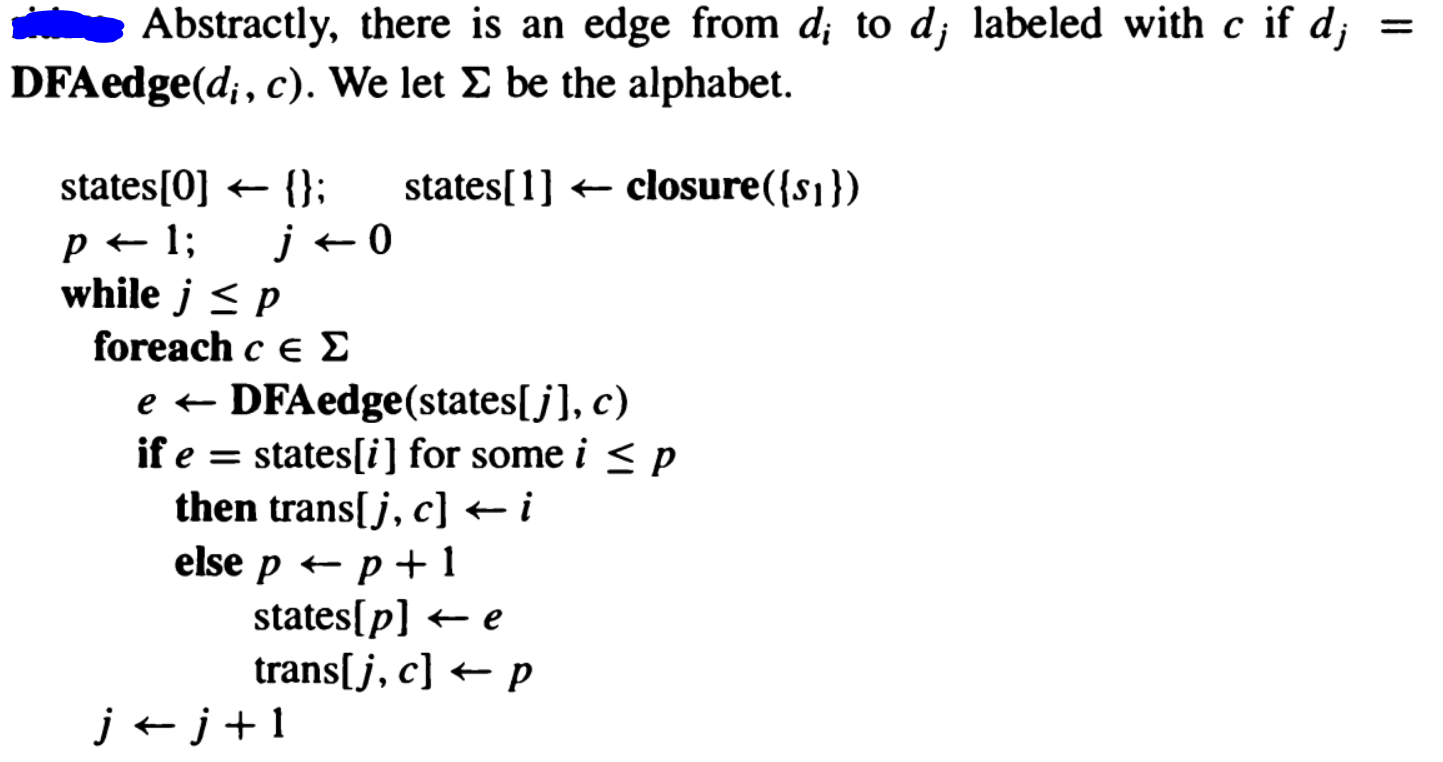
\includegraphics[width=0.5\textwidth,height=0.5\textheight,keepaspectratio]{nfa2}

DFA construction is a mechanical task easily performed by computer, so it 
makes sense to have an automatic lexical analyzer generator to translate  
regular expressions into a DFA. 

ML-Lex is a lexical analyzer generator that produces an ML program from 
a lexical specification. 

For each token type in the programming language to 
be lexically analyzed, the specification contains a regular expression and an 
action. The action communicates the token type (perhaps along with other 
information) to the next phase of the compiler. 

The output of ML-Lex is a program in ML - a lexical analyzer that  
interprets a DFA using the algorithm described in Section 2.3 and executes the 
action fragments on each match. The action fragments are just ML statements 
that return token values. 

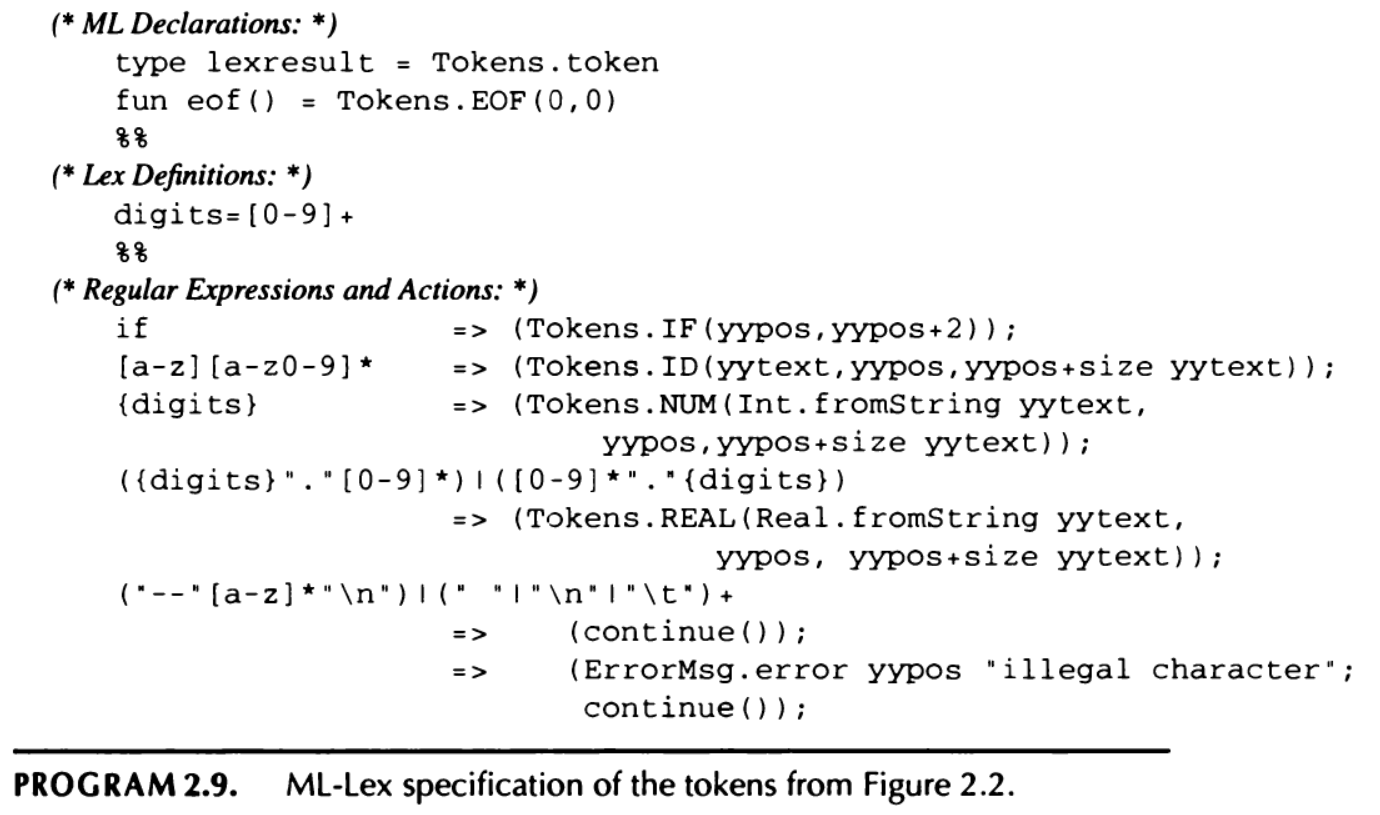
\includegraphics[width=0.5\textwidth,height=0.5\textheight,keepaspectratio]{lex}

The format is: user declarations \%\% ML-Lex definitions \%\% rules

The first part of the specification, above the first \%\% mark, contains  
functions and types written in ML. These must include the type lexresult, 
which is the result type of each call to the lexing function; and the  
function eof, which the lexing engine will call at end of file. This section can 
also contain utility functions for the use of the semantic actions in the third 
section. It is called with the same argument as lex (see \%arg, below), and must return a value of type lexresult. 

The second part of the specification contains regular-expression  
abbreviations and state declarations. For example, the declaration digits=$[0-9]^+$ 
in this section allows the name \{digits\} to stand for a nonempty sequence 
of digits within regular expressions. 

In the definitions section, the user can define named regular expressions, a set of start states, and specify which of the various bells and whistles of ML-Lex are desired.

The third part contains regular expressions and actions. The actions are 
fragments of ordinary ML code. Each action must return a value of type 
lexresult. In this specification, lexresult is a token from the Tokens 
structure. 

In the action fragments, several special variables are available. The string 
matched by the regular expression is yytext. The file position of the  
beginning of the matched string is yypos. The function continue () calls the 
lexical analyzer recursively. 

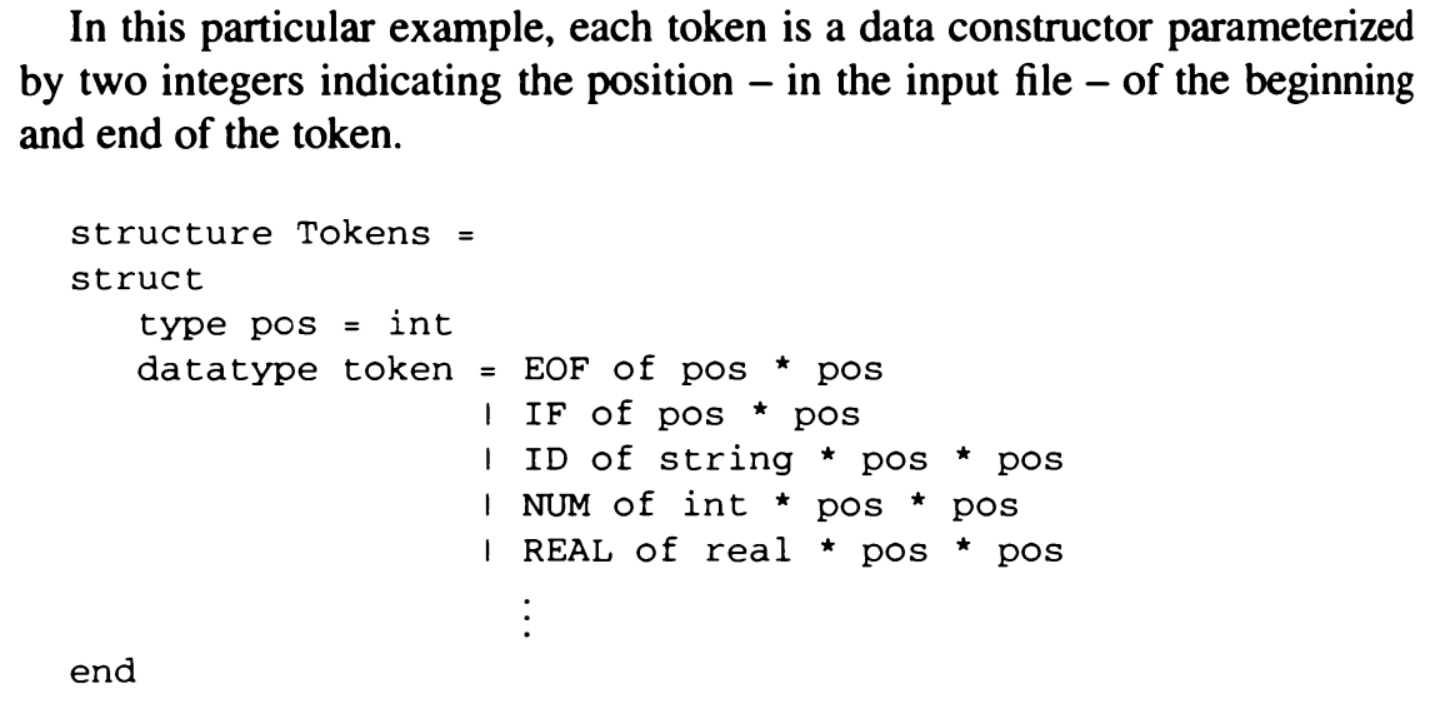
\includegraphics[width=0.5\textwidth,height=0.5\textheight,keepaspectratio]{lex2}

Arguments given to token are called payload.

The tokens are defined by the combined effect of
1. The \%term commands used in the ML-Yacc declaration section of your ML-Yacc
specification. These may add extra values to the token function’s argument and
thus extend the payload.
2. The lexresult type declaration in the user declarations of your ML-Lex specification

If a token has been defined by the \%term command in the .yacc file with no type,
then its payload is usually two integers - its the \%pos declaration which says so, see
chapter 9.4.3 on page 22. For example, looking at the SML/NJ compiler, we see that
the semicolon is defined by the ML-Yacc \%term command in file ml.grm as SEMICOLON.
There is no type specification. The payload is two integers specifying the character
positions in the source file of the start and end of the semicolon:
\begin{minted}{SML}
<INITIAL>";" => (Tokens.SEMICOLON(yypos,yypos+1));
\end{minted}
If a token has been defined in ML-Yacc with a type, then its payload will be a value
of that type, followed by two integers - again, its the \%pos declaration which calls for
those two integers, see chapter 9.4.3 on page 22.. For example, looking at the SML/NJ
compiler, we see that a real number is defined by the ML-Yacc \%term command in file
ml.grm as REAL of string. The payload is therefore a string followed by two integers
specifying the character position in the source file of the start and end of the real number:
\begin{minted}{SML}
<INITIAL>{real} => (Tokens.REAL(yytext,
yypos,
yypos+size yytext));
\end{minted}

But sometimes the step-by-step, state-transition model of automata is  
appropriate. ML-Lex has a mechanism to mix states with regular expressions. 
One can declare a set of start states; each regular expression can be prefixed 
by the set of start states in which it is valid. The action fragments can  
explicitly change the start state. In effect, we have a finite automaton whose edges 
are labeled, not by single symbols, but by regular expressions. This example 
shows a language with simple identifiers, if tokens, and comments delimited 
by (* and *) brackets: 

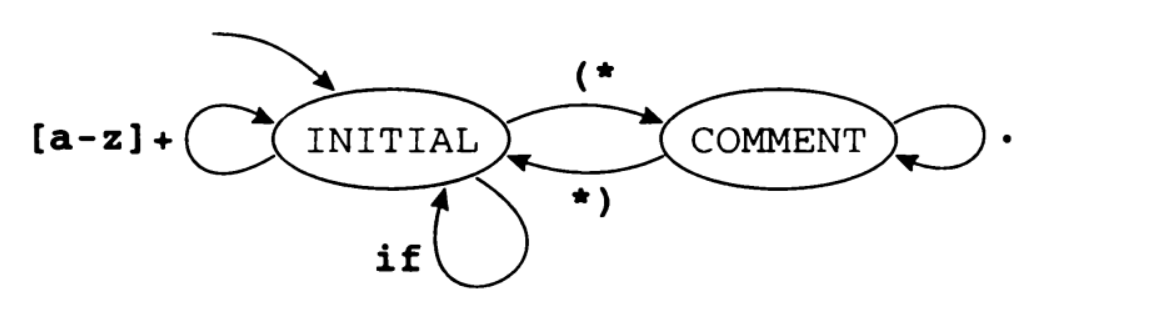
\includegraphics[width=0.5\textwidth,height=0.5\textheight,keepaspectratio]{lex3}

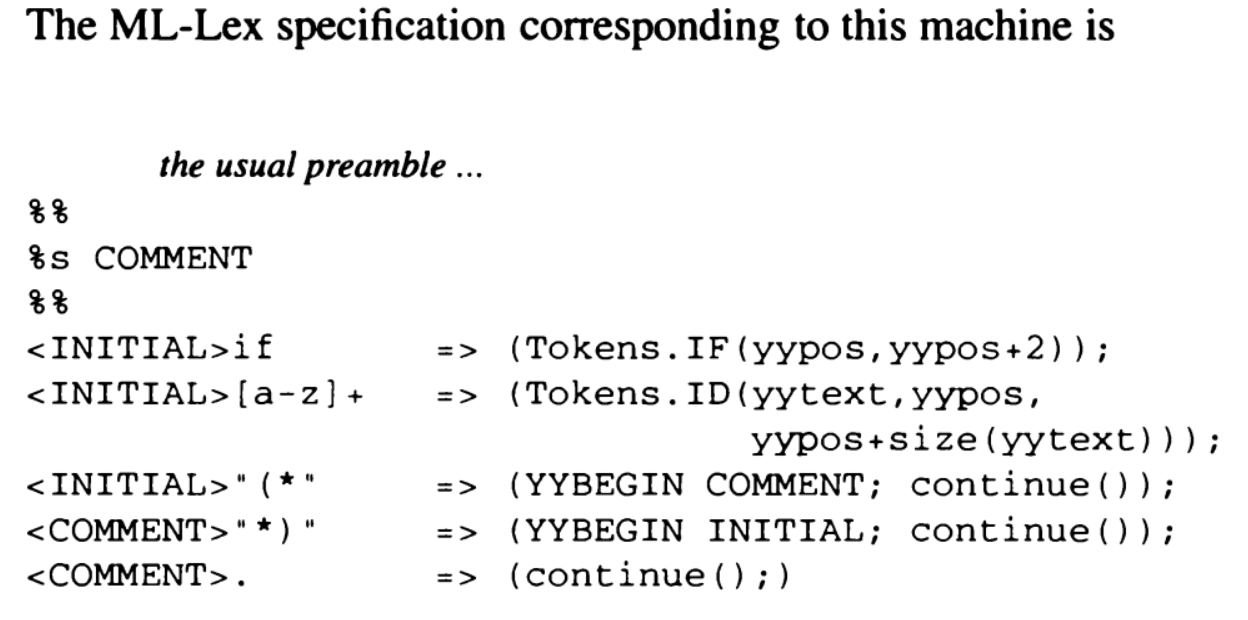
\includegraphics[width=0.5\textwidth,height=0.5\textheight,keepaspectratio]{lex4}

This example can be easily augmented to handle nested comments, via a 
global variable that is incremented and decremented in the semantic actions. 

Any regular expression not prefixed by a $<state>$ operates in all states; this  
feature is rarely useful. 

The alphabet for ML-Lex is the Ascii character set (character codes 0-127; or if %full is used, 0-255).

Certain rules
\begin{itemize}
    \item     An individual character stands for itself, except for the reserved characters 
    \begin{minted}{cpp}
    // ? * + | ( ) ^ $ / ; . = < > [ { " \

    \end{minted}

    \item A backslash followed by one of the reserved characters stands for that character. 

    \item Inside the brackets, only the symbols \begin{minted}{cpp} 
    \ - ^ 
\end{minted}
 are reserved. An initial up-arrow \^{} stands for the complement of the characters listed, e.g. [\^{}abc] stands any character except a, b, or c.
    \item  To include \^{} literally in a bracketed set, put it anywhere but first; to include - literally in a set, put it first or last. 
    \item The dot . character stands for any character except newline, i.e. the same as \begin{minted}{cpp}
        [^\n]
    \end{minted}
    \item The following special escape sequences are available, inside or outside of square brackets: 
    \begin{minted}{SML}
    \b backspace
    \n newline
    \t horizontal tab
    \ddd where ddd is a 3 digit decimal escape
    \end{minted}
    \item Any regular expression may be enclosed in parentheses ( ) for syntactic (but, as
    usual, not semantic) effect
    \item A sequence of characters will stand for itself (reserved characters will be taken literally) if it is enclosed in double quotes " ".
    \item A postfix repetition range \{a, b\} where a and b are small integers stands for any number of repetitions between a and b of the preceding expression. The notation \{a\} stands for exactly a repetitions. Ex: [0-9]\{3\}
    Any three-digit decimal number. 
    \item The rules should match all possible input. If some input occurs that does not match any rule, the lexer created by ML-Lex will raise an exception LexError.
    \item  The user may recursively call the lexing function with lex(). (If \%arg is used, the lexing function may be re-invoked with the same argument by using continue().) This is convenient for ignoring white space or comments silently:
    \begin{minted}{SML}
    [\ \t\n]+       => ( lex());
    \end{minted}
    \item To switch start states, the user may call YYBEGIN with the name of a start state. 
    \item If the lexer is to be used with the ML-Yacc parser, then additional glue declarations
    are needed:
    \begin{minted}{SML}
    5 structure T = Tokens
    6 type pos = int (* Position in file *)
    7 type svalue = T.svalue
    8 type (’a,’b) token = (’a,’b) T.token
    9 type lexresult = (svalue,pos) token
    10 type lexarg = string
    11 type arg = lexarg
    12 val linep = ref 1; (* Line pointer *)
    \end{minted}
    Lines 5 through 9 provide the basic glue. On line 9, lexresult returns the type of the
result returned by the rule actions.
If you are passing a parameter to the lexer, then you also need the additional glue
in lines 10 through 11. The lexer offers the possibility of counting lines using value yylineno described in
chapter 7.3.6. If you prefer to do this yourself with variable linep, you will need the
declaration on line 12
    \item Running ML - Lex file: From the Unix shell, run \begin{minted}{SML} 
        sml-lex myfile.lex 
        The output file will be myfile.lex.sml. The extension .lex is not required but is recommended. 
    \end{minted}
\end{itemize}

To get messages for lexer errors and unwelcome characters (note: l1 is the lineno. and l2 is the position in that line):
\begin{minted}{SML}
val error : string * int * int -> unit = fn
(e,l1,l2) => TextIO.output(TextIO.stdOut,"lex:line "
^Int.toString l1^" l2="^Int.toString l2
^": "^e^"\n")
val badCh : string * string * int * int -> unit = fn
(fileName,bad,line,col) =>
TextIO.output(TextIO.stdOut,fileName^"["
^Int.toString line^"."^Int.toString col
^"] Invalid character \""^bad^"\"\n");
\end{minted}

A typical error is to
forget to close an ongoing comment. If you allow ML style nested comments (* ... (*
... *) ... *) then you will need some management of nested comments and possible
end-of-file errors in the lexer. 
\begin{minted}{SML}
    21 val mlCommentStack : (string*int) list ref = ref [];
    22 val eof = fn fileName =>
    23 (if (!mlCommentStack)=[] then ()
    24 else let val (file,line) = hd (!mlCommentStack)
    25 in TextIO.output(TextIO.stdOut,
    26 " I am surprized to find the
    27 ^" end of file \""fileName^"\"\n"
    28 ^" in a block comment which began"
    29 ^" at "^file^"["^Int.toString line^"].\n")
    30 end;
    31 T.EOF(!linep,!linep));
\end{minted}

It assumes that the ML-Lex command \%arg, chapter 7.2.7, has
been specified and the name of the source file fileName has been passed to the lexer,
see line 417 on page 43. If this is not the case, then fileName is replaced by (). For
this treatment of nested commands to work well, additional measures are needed for the
ends of lines in the rules section 7.3


The ML-Lex definitions section provides the following commands. They are all terminated with a semicolon ;

Use the specified code to create a functor header for the lexer structure. For example, if
you are using ML-Yacc and you have specified \%name My in the ML-Yacc declarations:
\begin{minted}{SML}
65 %header (functor MyLexFun(structure Tokens: My_TOKENS));
\end{minted}
This has the effect of turning what would have been a structure into a functor. The
functor is needed for the glue code which integrates the lexer into a project.
The SML/NJ compiler uses this technique with ML in place of My. Our working
example also uses the technique with Pi in place of My. See lines 317 on page 40 and
391 on page 42.
If you prefer to create the lexer as an SML/NJ structure, then omit this command
and use the command \%structure
If you prefer to create your lexer as an SML/NJ structure rather than a functor, when
for example you are not using ML-Yacc, then use the command \%structure identifier
to name the structure in the output program my.lex.sml as identifier instead of the
default Mlex

\%count counts newlines using yylineno

\%posarg
Pass an initial-position argument to function makeLexer. See 10.4.
\%arg
An extra (curried) formal parameter argument is to be passed to the lex functions, and
to the eof function in place of (). See 7.3.2. For example:
\begin{minted}{SML}
66 %arg (fileName:string);
\end{minted}
The argument value is passed in the call to the parser. See line 415 on page 43 

lex() and continue():
If \%arg, chapter 7.2.7, is not used, you may recursively call the lexing function with
lex().
\begin{minted}{SML}
82 [\ \t]+ => ( lex() );
\end{minted}
For example, line 82 ignores spaces and tabs silently;
However, if \%arg is used, the lexing function may be re-invoked with the same argument by using continue().
\begin{minted}{SML}
83 <COMMENT>. => (continue());
\end{minted}
For example, line 83 silently ignores all characters except a newline when the parser is
in the user-defined state COMMENT

yylineno: 
The value yylineno is defined only if command \%count has been specified, chapter 7.2.5.
yylineno provides the current line number.
7.3.6.1 Warning This function should be used only if it is really needed. Adding
the yylineno facility to a lexer will slow it down by 20\%. It is much more efficient to
recognise nn and have an action that increments a line-number variable. For example,
see chapter 11.2.3 on page 38 in our working example.
\begin{minted}{SML}
datatype lexresult= DIV | EOF | EOS | ID of string | LPAREN |
NUM of int | PLUS | PRINT | RPAREN | SUB | TIMES 

val linenum = ref 1
val error = fn x => output(std_out,x ^ "\n")
val eof = fn () => EOF
%%
%structure CalcLex
alpha=[A-Za-z];
digit=[0-9];
ws = [\ \t];
%%
\n       => (inc linenum; lex());
{ws}+    => (lex());
"/"      => (DIV);
";"      => (EOS);
"("      => (LPAREN);
(* revfold ((('a * 'b)->'b) ->'a list ->'b -> 'b) is like fold done from backwards (in this case from left) explode will convert the string to list of characters. *)
{digit}+ => (NUM (revfold (fn(a,r)=>ord(a)-ord("0")+10*r) (explode yytext) 0));
")"      => (RPAREN);
"+"      => (PLUS);
{alpha}+ => (if yytext="print" then PRINT else ID yytext);
"-"      => (SUB);
"*"      => (TIMES);
.        => (error ("calc: ignoring bad character "^yytext); lex());
\end{minted}
\section{Parsing}
The parser returns an abstract syntax tree of the expression being evaluated. The parser gets tokens from the scanner to parse the input and build the AST. When an AST is
returned by the parser, the compiler calls the code generator to evaluate the tree and produce the target code.

There are two main parts to a compiler, the front end and back end. The front end
reads the tokens and builds an AST of a program. The back end generates the code
given the AST representation of the program. As presented in earlier chapters, the
front end consists of the scanner and the parser.
\end{document}